\pgfdeclarelayer{background}
\pgfsetlayers{background,main}

\def\scale{0.62}

\colorlet{circle edge}{black!50}

\tikzset{
  filled/.style={fill=circle area, draw=circle edge, thick},  outline/.style={draw=circle edge, thick}
  }

\setlength{\parskip}{5mm}

\tikzstyle{edge} = [draw, thick, -]
\tikzstyle{vertex}=[circle,fill=black!25,minimum size=10pt,inner sep=0pt]

\tikzstyle{selected edge} = [draw,line width=5pt,-,gray!50]
\tikzstyle{ignored edge} = [draw,line width=5pt,-,black!20]

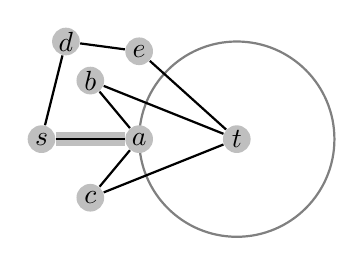
\begin{tikzpicture}[scale=\scale]
    % We put this last to ensure that it is not overwritten
    \draw[outline] {(4, 0) circle (2cm)} node {};

    \foreach \pos/\name in {{(0, 0)/s}, {(2, 0)/a}, {(0.5, 2)/d}, {(2, 1.8)/e},  {(1, 1.2)/b}, {(1, -1.2)/c}, {(4,0)/t}}
      \node[vertex] (\name) at \pos {$\name$};
      
    \foreach \source/\sink in {s/a, s/d, a/b, a/c, b/t, c/t, d/e, e/t} 
      \path[edge] (\source) -- (\sink); 

    \begin{pgfonlayer}{background}
      \foreach \source/ \dest in {s/a}
          \path[selected edge] (\source) -- (\dest);
    \end{pgfonlayer}

\end{tikzpicture}
